% !TEX TS-program = pdflatex
% !TEX encoding = UTF-8 Unicode

% This is a simple template for a LaTeX document using the "article" class.
% See "book", "report", "letter" for other types of document.

\documentclass[10pt,onecolumn]{article}

\usepackage[utf8]{inputenc} % set input encoding (not needed with XeLaTeX)
\usepackage{graphicx}
\usepackage{listings} 
\usepackage{caption} 
\usepackage{xcolor,colortbl}
\usepackage{mathtools}
\usepackage{wrapfig}
\usepackage{tabularx}
\usepackage{pdflscape}

\graphicspath{ {figures/} }

%%% Examples of Article customizations
% These packages are optional, depending whether you want the features they provide.
% See the LaTeX Companion or other references for full information.

%%% PAGE DIMENSIONS
\usepackage{geometry} % to change the page dimensions
\geometry{a4paper} % or letterpaper (US) or a5paper or....
\geometry{margin=1in} % for example, change the margins to 2 inches all round
% \geometry{landscape} % set up the page for landscape
%   read geometry.pdf for detailed page layout information

\usepackage{graphicx} % support the \includegraphics command and options

% \usepackage[parfill]{parskip} % Activate to begin paragraphs with an empty line rather than an indent

%%% PACKAGES
\usepackage{polski}
\usepackage{booktabs} % for much better looking tables
\usepackage{array} % for better arrays (eg matrices) in maths
\usepackage{paralist} % very flexible & customisable lists (eg. enumerate/itemize, etc.)
\usepackage{verbatim} % adds environment for commenting out blocks of text & for better verbatim
\usepackage{subfig} % make it possible to include more than one captioned figure/table in a single float
\usepackage{indentfirst}
\usepackage{amsfonts}
\usepackage{amssymb}
\usepackage{amsthm}
\usepackage{subfig}

\newtheorem{theorem}{Twierdzenie}
\theoremstyle{definition}
\newtheorem{definition}{Definicja}
\theoremstyle{hypothesis}
\newtheorem{hypothesis}{Hipoteza}
\theoremstyle{capability}
\newtheorem{capability}{Własność}
\newtheorem{lemma}[theorem]{Lemat}

% These packages are all incorporated in the memoir class to one degree or another...

%%% HEADERS & FOOTERS
\usepackage{fancyhdr} % This should be set AFTER setting up the page geometry
\pagestyle{fancy} % options: empty , plain , fancy
\renewcommand{\headrulewidth}{0pt} % customise the layout...
\lhead{}\chead{}\rhead{}
\lfoot{}\cfoot{\thepage}\rfoot{}

%%% SECTION TITLE APPEARANCE
\usepackage{sectsty}
\allsectionsfont{\sffamily\mdseries\upshape} % (See the fntguide.pdf for font help)
% (This matches ConTeXt defaults)

%%% ToC (table of contents) APPEARANCE
\usepackage[nottoc,notlof,notlot]{tocbibind} % Put the bibliography in the ToC
\usepackage[titles,subfigure]{tocloft} % Alter the style of the Table of Contents
\renewcommand{\cftsecfont}{\rmfamily\mdseries\upshape}
\renewcommand{\cftsecpagefont}{\rmfamily\mdseries\upshape} % No bold!
\setlength{\parindent}{0.5cm} 

%%% END Article customizations

%%% The "real" document content comes below...

\definecolor{Gray}{gray}{0.85}
\definecolor{LightCyan}{rgb}{0.88,1,1}
\newcolumntype{a}{>{\columncolor{Gray}}c}
\newcolumntype{b}{>{\columncolor{white}}c}

\newcommand{\subsubfloat}[2]{%
  \begin{tabular}{@{}c@{}}#1\\#2\end{tabular}%
}

\begin{document}

%=============================================
% STRONA TYTULOWA
%=============================================

\begin{titlepage}
	\centering
	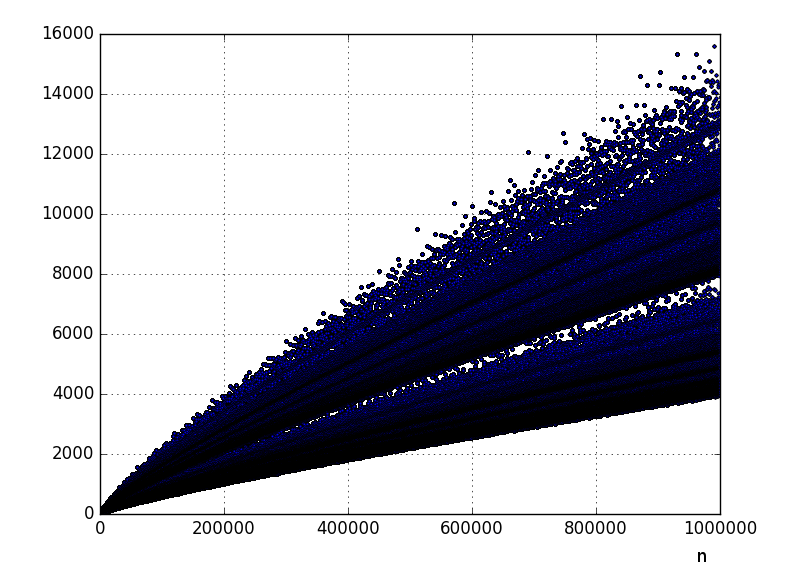
\includegraphics[width=0.8\textwidth]{title_page}\par\vspace{1cm}
	\vspace{1.5cm}
	{\huge\bfseries Tajemnice Liczb Pierwszych\par}
	\vspace{2cm}
	{\Large\itshape Marcin Barylski\par}
	\vfill

\title{}
\end{titlepage}

%=============================================
% SPIS TREŚCI
%=============================================

\tableofcontents

\newpage

%=============================================
% WPROWADZENIE
%=============================================

\section{Wprowadzenie}

\subsection{Podzielność liczb}

\begin{definition}[O dzieleniu liczba całkowitych]
Niech $a$, $b$ $\in$ $\mathbb{Z}$. Mówimy, że $a$ dzieli $b$, zapisując $a$ $\mid$ $b$, jeśli istnieje $c$ $\in$ $\mathbb{Z}$ takie, że $a \times c = b$. W takim wypadku mówimy, że $a$ jest dzielnikiem $b$. Mówimy także, że $a$ nie dzieli $b$, zapisując $a$ $\nmid$ $b$, jeśli nie ma takiego $c$ $\in$ $\mathbb{Z}$, że $a \times c = b$.
\end{definition}

Jeśli $a \mid b$, to liczbę $b$ nazywamy wielokrotnością liczby $a$.

\begin{definition}[O dzielniku właściwym]
Dzielnikiem właściwym liczby całkowitej $b$ nazywamy liczbę naturalną $a$ taką, że $a$ $\mid$ $b$ oraz $a \textless b$.
\end{definition}

\begin{definition}[O największym wspólnym dzielniku]
Największym wspólnym dzielnikiem liczb całkowitych $a$ i $b$ nazywamy największą liczbę $d$ taką, że $d$ $\mid$ $a$ i $d$ $\mid$ $b$, zapisując to $NWD(a, b) = d$.
\end{definition}

Definicję *O największym wspólnym dzielniku*, za pomocą indukcji matematycznej, można rozszerzyć na dowolną, skończoną liczbę argumentów w $NWD()$.

\subsection{Liczby pierwsze}

\begin{definition}[O liczbie pierwszej]
Liczba całkowita $n$ \textgreater 1 jest liczbą pierwszą, jeśli jej jedynymi dodatnimi dzielnikami są 1 oraz $n$. 
\end{definition}

Definicję *O liczbie pierwszej* można też wyrazić w inny, komplementarny sposób: liczba całkowita $n$ \textgreater 1 jest liczbą pierwszą, jeśli nie jest iloczynem dwóch liczb całkowitych \textgreater 1. Definicja taka akcentuje różnicę liczby pierwszej w porównaniu z liczbą złożoną, która jest iloczynem przynajmniej dwóch liczb całkowitych \textgreater 1. Liczba pierwsza ma dokładnie jeden dzielnik \textgreater 1, równy jej samej. Przykładowo, liczba 11 jest liczbą pierwszą, bowiem jej jedynymi dzielnikami są 1 i 11. Sekwencja OEIS A000040 przedstawia początkowe liczby pierwsze.

\begin{capability}[Każda liczba pierwsza ma tylko jeden dzielnik właściwy]
Jedynym dzielnikiem właściwym liczby pierwszej jest 1.
\end{capability}

Własność *Każda liczba pierwsza ma tylko jeden dzielnik właściwy* wynika z definicji *O liczbie pierwszej* i *O dzielniku właściwym*.

\begin{capability}[Tylko jedna liczba pierwsza jest parzysta]
Istnieje tylko jedna liczba pierwsza parzysta, 2.
\end{capability}

Nie może istnieć inna niż 2 liczba parzysta pierwsza, bowiem każda liczba parzysta jest podzielna przez $2$, a jeśli jest większa niż $2$, to posiada przynajmniej jeszcze jeden dzielnik różny od $1$ i $2$. Zatem wśród liczb parzystych istnieje dokładnie jedna liczba, która spełnia definicję *O liczbie pierwszej* i jest nią $2$.

\begin{capability}[Druga i każda kolejna liczba pierwsza są nieparzyste]
Wszystkie liczby pierwsze większe od 2 są nieparzyste.
\end{capability}

Wynika to bezpośrednio z własności *Tylko jedna liczba pierwsza jest parzysta*. Istnieją kolejne liczby pierwsze: $3$, $5$, $7$, \ldots i wszystkie są nieparzyste.

\subsection{Liczby pierwsze bliźniacze}

\begin{definition}[O liczbach pierwszych bliźniaczych]
Liczby pierwsze bliźniacze to takie liczby pierwsze, między którymi różnica wynosi 2. Mniejsza z tych liczb nazywana jest mniejszą liczbą bliźniaczą, zaś druga - większą liczbą bliźniaczą.
\end{definition}

Sekwencja OEIS A014574 przedstawia początkowe liczby bliźniacze w postaci $n \pm 1$, zaś sekwencje OEIS A001359 i OEIS A006512 kolejno początkowe mniejsze liczby pierwszy bliżniacze i większe liczby pierwsze bliźniacze.

\begin{lemma}[5 jest jedyną liczbą pierwszą bliźniaczą z dwoma różnymi liczbami pierwszymi]
Liczba pierwsza 5 jest jedyną liczbą, która jest zarówno liczbą pierwszą bliźniaczą mniejszą (w parze z 7) i liczbą pierwszą bliźniaczą większą (w parze z 3).
\end{lemma}
\begin{proof}
W sekwencji liczb $n, n+2, n+4$ jedna jest zawsze podzielna przez $3$. $n+2$ jest zarazem mniejszą liczbą pierwszą bliźniaczą jak i większą liczbą pierwszą bliźniaczą wtedy i tylko wtedy, gdy wszystkie z liczb $n, n+2, n+4$ są pierwsze. $3$ jest jedyną liczbą pierwszą podzielną przez $3$, tak więc $3$ musi występować w sekwencji $n, n+2, n+4$. $3$ musi być pierwszą liczbą w tej sekwencji, bowiem dwie inne możliwe kombinacje: $1, 3, 5$ oraz $-1, 1, 3$ nie zawierają wyłącznie liczb pierwszych. To oznacza, że jedyną dozwoloną sekwencją jest $3, 5, 7$ oraz $5$ jest jedyną liczbą pierwszą, którą jest liczbą pierwszą bliźniaczą w dwóch parach: $(3, 5)$ i $(5, 7)$.
\end{proof}

\subsection{Liczby względnie pierwsze}

\begin{definition}[O liczbach względnie pierwszych]
Liczby całkowite nazywami względnie pierwszymi, jeśli ich największym wspólnym dzielnikiem (NWD) jest 1.
\end{definition}

Fakt, że liczby $x, y, \dots , z$ są względnie pierwsze, zapisuje się symbolicznie jako $NWD (x, y,\dots ,z)=1$. 

\begin{capability}[Największy wspólny dzielnik liczb, które nie są względnie pierwsze]
Jeśli liczby całkowite $x$, $y$, \dots, $z$ nie są względnie pierwsze, to $NWD (x, y,\dots ,z) = d \textgreater 1$, zaś $d$ jest liczbą pierwszą bądź iloczynem liczb pierwszych.
\end{capability}

\begin{capability}[Najmniejsza wspólna wielokrotność liczb względnie pierwszych]
Jeśli liczby całkowite $x$ i $y$ są względnie pierwsze, to $NWW (x, y) = x \times y$.
\end{capability}

\subsection{Liczby złożone}

\begin{definition} [O liczbie złożonej]
Liczba całkowita $n$ \textgreater 1 jest liczbą złożoną, jeśli nie jest liczbą pierwszą.
\end{definition}

Liczby $0$ oraz $1$ nie są ani liczbami pierwszymi, ani złożonymi, choć w przeszłości traktowano $1$ jako liczbę pierwszą. Obecnie $1$ nie jest uważana za liczbą pierwszą, gdyż wyłączenie jej ze zbioru liczb pierwszych uprościło *Fundamentalne twierdzenie arytmetyki*, w którym unikatowość rozkładu dowolnej liczby dodatniej \textgreater $1$ na iloczyn liczb pierwszych nie jest zakłócony przez $1$ $\times$ $1$ $\times$ $\ldots$ $\times$ $1$. Zauważmy też, że jeśli spojrzymy na liczbę dzielników $0$ i $1$, to stwierdzimy, że liczby te nie pasują ani do zbioru liczb pierwszych, ani złożonych. $0$ ma nieskończenie wiele dzielników (każda liczba całkowita $\textgreater 1$ dzieli $0$), zaś $1$ ma dokładnie jeden dzielnik ($1$). Wszystkie liczby pierwsze mają dokładnie dwa dzielniki (siebie samą i $1$), zaś wszystkie liczby złożone - skończoną liczbę dzielników, większą od $2$.

\subsection{Dzielniki pierwsze}

Przyjrzyjmy się bliżej dzielnikom liczb naturalnych.

\begin{theorem} [O co najmniej jednym dzielniku pierwszym liczby całkowitej większej od jedności]
Każda liczba całkowita $n$ \textgreater 1 ma co najmniej jeden dzielnik, który jest liczbą pierwszą. 
\end{theorem}
 
\begin{proof}
Niech $n$ jest liczbą całkowitą \textgreater 1. $n$ ma zawsze dzielniki \textgreater 1 - jednym z nich jest $n$.  Wśród dzielników liczby $n$, które są \textgreater 1, zawsze istnieje najmniejszy dzielnik, $p$. Gdyby $p$ nie było liczbą pierwszą, to zgodnie z definicją *O liczbie pierwszej* $p$ byłoby iloczynem dwóch liczb całkowitych $a$ i $b$, obu \textgreater 1, $p = a \times b$. Zarówno $a$ jak i $b$ byłyby mniejsze niż $p$, co jest wbrew definicji $p$.
\end{proof}

\begin{theorem} [O co najmniej jednym dzielniku pierwszym liczby złożonej mniejszym lub równym niż pierwiastek kwadratowy z liczby]
Każda liczba złożona $n$ \textgreater 1 ma co najmniej jeden dzielnik $\le$ $\sqrt{n}$, który jest liczbą pierwszą. 
\end{theorem}
 
\begin{proof}
Jeśli $n$ jest liczbą złożoną, to istnieją dwie takie liczby całkowite dodatnie $a$ i $b$ ($a \leq b$), obie mniejsze niż $n$, że: $n = a \times b$. Zatem: $n = a \times b \geq a^2$, skąd wynika, po pierwiastkowaniu obu stron nierówności, że: $a \leq \sqrt{n}$. Liczba $a$ jest \textgreater 1, w przeciwnym razie $b$ nie byłoby mniejsze niż $n$. Zgodnie z twierdzeniem *O co najmniej jednym dzielniku pierwszym liczby całkowitej* liczba $a$ ma dzielnik pierwszy $p$. $p$ jest dzielnikiem dzielnika $a$ liczby $n$, więc $p$ jest też dzielnikiem $n$. $p \leq a \leq \sqrt{n}$, stąd: $p \leq \sqrt{n}$.
\end{proof}

\newpage

%=============================================
% LICZBY PIERWSZE JAKO BUDULEC INNYCH LICZB
%=============================================

\section{Liczby pierwsze jako budulec innych liczb}

\subsection{Liczby naturalne zbudowane z liczb pierwszych}

Zastanówmy się nad reprezentacją dowolnej liczby naturalnej poprzez liczby pierwsze.

\begin{theorem}[Fundamentalne twierdzenie arytmetyki]
Każda liczba całkowita $n$ \textgreater 1 może zostać zapisana jako iloczyn skończonej liczby liczb pierwszych $p_1$, $p_2$, $p_3$, $\ldots$ , $p_n$, tzn.: $$ n = p_1 \times p_2 \times p_3 \times \ldots \times p_n$$  Rozkład liczby $n$ jest unikatowy, jeśli $p_i$ są uporządkowane w tym rozkładzie, tzn. $p_1$ $\leq$ $p_2$ $\leq$ $\ldots$ $\leq$ $p_n$.
\end{theorem}
 
\begin{proof}
TBD
\end{proof}

\subsection{Liczby doskonałe zbudowane z liczb pierwszych}

Już od czasów starożytnych niektóre liczby uważane były za wyjątkowe. Szczególnie dużo uwagi poświęcano liczbom doskonałym. Euklides opisał je w Elementach, w księdze IX \cite{euklides}.

\begin{definition} [O liczbie doskonałej]
Liczbą doskonałą nazywamy liczbę naturalną, która jest sumą wszystkich swoich dzielników właściwych.
\end{definition}

Liczba $6$ jest najmniejszą liczbą doskonałą, bowiem zbiorem jej dzielników właściwych jest $\lbrace 1, 2, 3 \rbrace$ oraz $6 = 1 + 2 +3$. Sekwencja OEIS A000396 przedstawia 10 pierwszych liczb doskonałych.
Wszystkie znane liczby doskonałe są parzyste. Nie wiadomo, czy istnieją nieparzyste liczby doskonałe. Jeśli taka liczba istnieje, to musi być wiekszą od $10^{1500}$ \cite{ochemrao2012}. Euler pokazał, że nieparzysta liczba doskonała, jeśli istnieje, musi mieć postać $N = p^{4a+1} \times Q^2$, gdzie $p$ jest liczbą pierwszą postaci $4 \times k+1$ ($a, k \in \mathbb{N}$).

\begin{theorem}[O parzystych liczbach doskonałych]
Każda parzysta liczba doskonała jest postaci $(2^p - 1) \times 2^{p - 1}$, gdzie $2^p - 1$ jest liczbą pierwszą.
\end{theorem}

\begin{proof}
TBD
\end{proof}

\subsection{Liczby pierwsze Mersenne'a}

\begin{definition} [O liczbach Mersenne'a]
Liczbami Mersenna $M_p$ nazywamy liczby postaci $2^p - 1$, gdzie $p$ jest liczbą naturalną.
\end{definition}

\begin{theorem}[Warunek konieczny pierwszości liczb Mersenne'a]
Warunkiem koniecznym, aby liczba Mersenne'a $2^p - 1$ była pierwsza jest to, aby $p$ było liczbą pierwszą.
\end{theorem}

\begin{proof}
Niech $n$ będzie dodatnią liczbą złożoną, tzn. istnieją $a, b \in \mathbb{N} \textgreater 1$, że $n = a \times b$. Wtedy: $M_n = 2^n - 1 = 2^{ab} - 1 = (2^a)^b - 1^b = (2^a - 1)(2^{a(b - 1)} + 2^{a(b - 2)} + \ldots + 2^{a(b-b)})$. Oznacza to, że liczba $M_n$ jest złożona, bo w jej rozkładzie są dwa czynniki $\textgreater 1$.
\end{proof}

Niestety, pierwszość wykładnika $p$ w liczbie Mersenne'a $M_p$ nie jest warunkiem wystarczającym pierwszości $M_p$ (kontrprzykład: $M_{11} = 2^{11} - 1 = 23 \times 89$). Otwarte pozostają również dwie hipotezy (hipoteza $\ref{Mers_comp_prime_index_inf}$ i hipoteza $\ref{Mers_prime_inf}$), tzn. nie wiemy, czy istnieje nieskończenie wiele złożonych liczb Mersenne'a o wykładnikach pierwszych oraz czy pierwszych liczb Mersenne'a jest nieskończenie wiele.

\begin{hypothesis}[O nieskończenie wielu złożonych liczb Mersenne'a o wykładnikach pierwszych]
Istnieje nieskończenie wiele złożonych liczb Mersenne'a $M_p = 2^p - 1$, gdzie $p$ jest liczbą pierwszą.
\label{Mers_comp_prime_index_inf}
\end{hypothesis}

\begin{hypothesis}[O nieskończenie wielu pierwszych liczb Mersenne'a]
Istnieje nieskończenie wiele pierwszych liczb Mersenne'a.
\label{Mers_prime_inf}
\end{hypothesis}

\subsection{Liczby parzyste zbudowane z liczb pierwszych}

W 1742 roku Christian Goldbach w swoim liście do Leonarda Eulera \cite{goldbach1742} wyraził przypuszczenie, że każda nieparzysta liczba naturalna \textgreater 5 może zostać przedstawiona jako suma trzech liczb pierwszych. W tych czasach traktowano liczbę 1 jako liczbę pierwszą. Euler uprościł tę hipotezę twierdząc, że każda liczba parzysta \textgreater 2 jest sumą dwóch liczb pierwszych. Choć finalny kształt hipotezie nadał Euler, nazywana jest ona Hipotezą Goldbacha. Hipoteza Goldbacha do dnia dzisiejszego nie została rozstrzygnięta i jest jednym z bardziej inspirujących problemów w teorii liczb, mających wpływ na rozwój matematyki w XX i XXI wieku. Wraz z hipotezą Riemanna widnieje na miejscu 8 listy Hilberta \cite{hilbert1900}, opisującej otwarte wyzwania matematyczne stojące u progu XX wieku.

\begin{wrapfigure}{hr}{0.5\textwidth}
  \begin{center}
    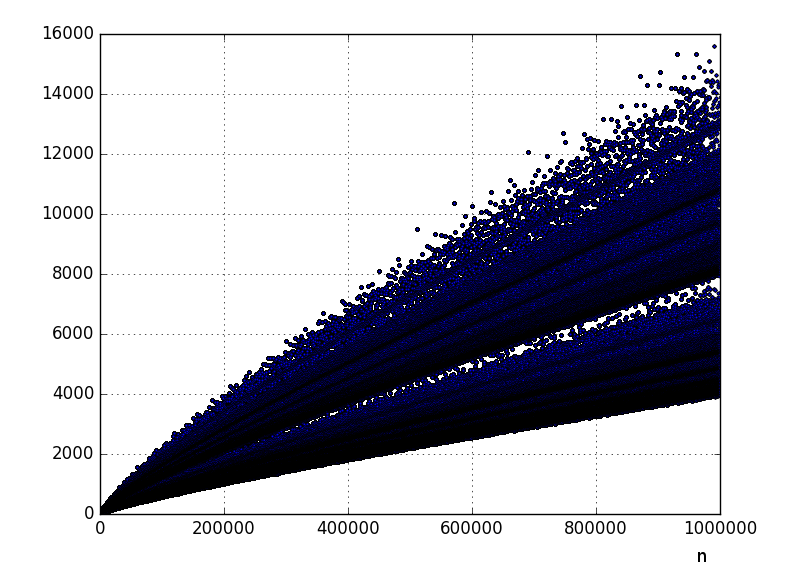
\includegraphics[width=0.48\textwidth]{f_goldbach_pairs}
  \end{center}
  \caption{Kometa Goldbacha - liczba możliwych rozkładów Goldbacha dla kolejnych dodatnich liczb parzystych - wykres funkcji $r(n)$ (2 \textless $n$ \textless $10^6$)}
  \label{fig:goldbach_pairs}
\end{wrapfigure}

\begin{hypothesis}[Hipoteza Goldbacha]
Każda liczba parzysta \textgreater 2 jest sumą dwóch liczb pierwszych.
\label{Goldbach_hyp}
\end{hypothesis}

Równolegle z szukaniem dowodu na prawdziwość hipotezy $\ref{Goldbach_hyp}$, wraz z rozwojem możliwości obliczeniowych komputerów, możliwe stało się jej potwierdzanie dla coraz to większych dodatnich liczb parzystych $n$. Hipoteza została dotychczas potwierdzona empirycznie dla wszystkich $n$ $\leq$ 4 $\times$ $10^{18}$ \cite{oliveira2012}. Dowodu matematycznego, uznanego przez społeczność matematyczną wciąż brak.\par

\begin{definition} [O rozkładzie Goldbacha]
Wyrażenie danej liczby parzystej $n$ \textgreater 2 jako sumy dwóch liczb pierwszych nosi nazwę rozkładu Goldbacha.
\end{definition}

Oznaczmy przez $R(n)$ zbiór wszystkich możliwych rozkładów Goldbacha dla $n$, zaś przez $r(n)$ - liczbę takich możliwych rozkładów dla $n$. 
Wykres $r(n)$ dla kolejnych $n$ tworzy tzw. kometę Goldbacha (Rysunek $\ref{fig:goldbach_pairs}$), ilustrującą rosnący trend dolnego oszacowania $r(n)$. Sekwencja A045917 przedstawia 98 pierwszych wyrazów $r(n)$.

\begin{figure}{hr}
\centering

\subfloat{
  \begin{minipage}{\columnwidth}\footnotesize
  \centering
  \subsubfloat{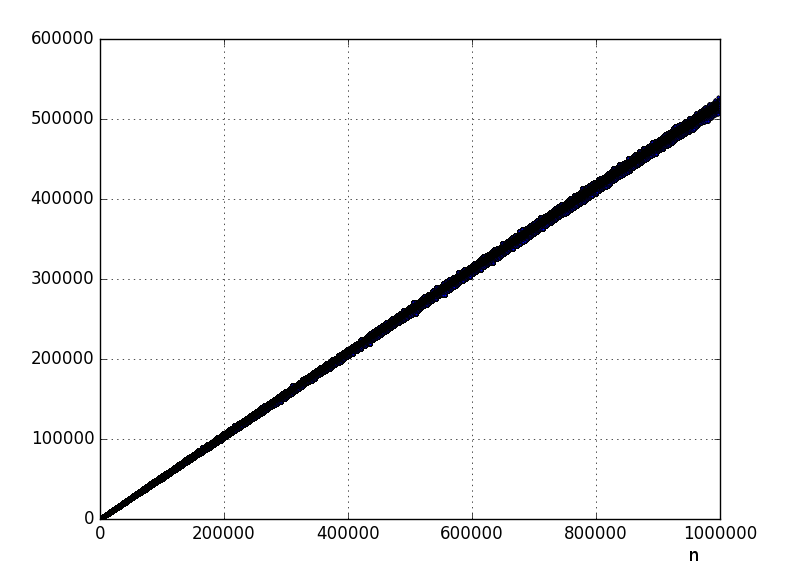
\includegraphics[width=0.45\columnwidth]{f_goldbach_avg_diff_pairs}}{a) Średnia różnica (arytmetyczna) w $R(n)$}%
  \qquad
  \subsubfloat{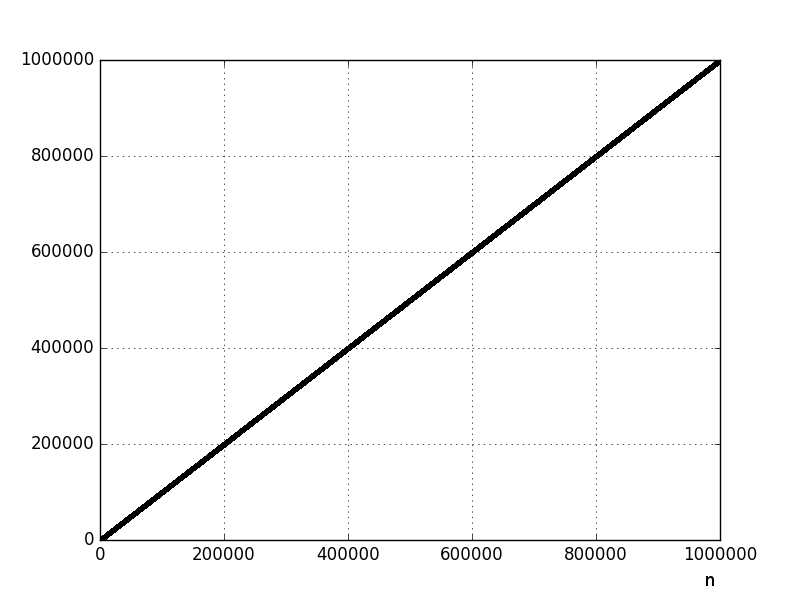
\includegraphics[width=0.45\columnwidth]{f_goldbach_max_diff_pairs}}{b) Największa różnica w $R(n)$}

  \medskip

  \subsubfloat{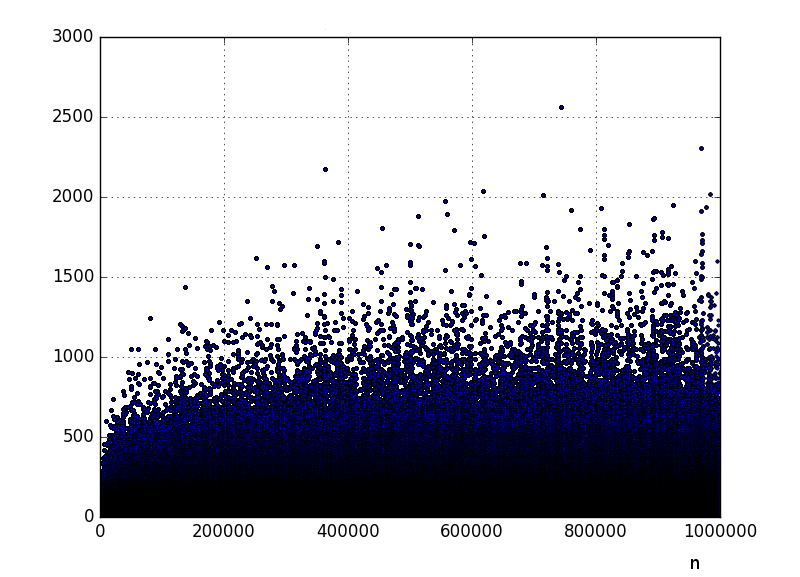
\includegraphics[width=0.45\columnwidth]{f_goldbach_min_diff_pairs}}{c) Najmniejsza różnica w $R(n)$}%
  \qquad
  \subsubfloat{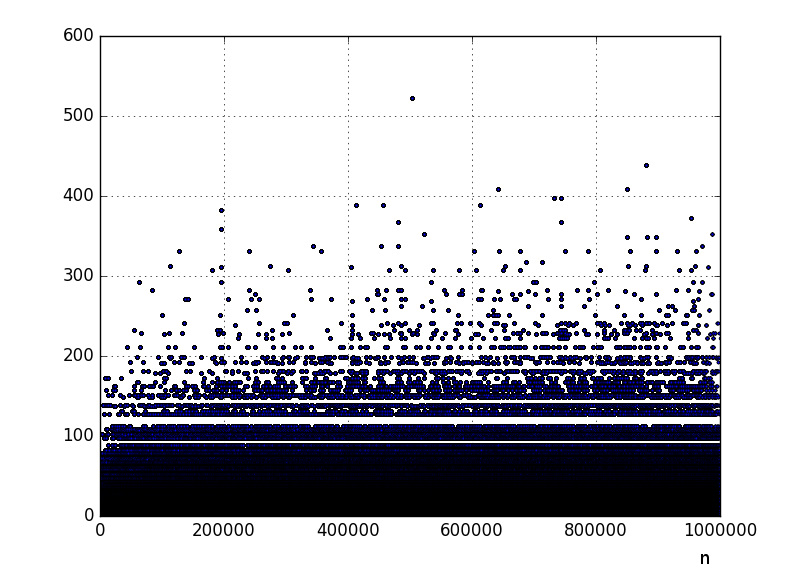
\includegraphics[width=0.45\columnwidth]{f_goldbach_min_prime_in_sum}}{d) Minimalna liczba pierwsza w $R(n)$}
  \end{minipage}}

\caption{Obserwacje dotyczące Hipotezy Goldbacha dla liczb parzystych 2 \textless $n$ \textless $10^6$}
\end{figure}

\subsection{Liczby nieparzyste zbudowane z liczb pierwszych}

Hipoteza Goldbacha stała się przyczynkiem do kolejnych rozważań na temat sum liczb pierwszych. Sformułowano m.in. *Słabą hipotezę Goldbacha*, która dotyczy liczb nieparzystych.

\begin{hypothesis}[Słaba hipoteza Goldbacha]
Każda liczba nieparzysta \textgreater 7 jest sumą trzech nieparzystych liczb pierwszych.
\label{Goldbach_weak_hyp}
\end{hypothesis}

Hipoteza nazywana jest słabą wersją hipotezy Goldbacha, bowiem dowodząc prawdziwość silnej hipotezy dowiedziemy prawdziwość hipotezy słabej. Wystarczy bowiem od liczby nieparzystej odjąć 3 (liczbę pierwszą), aby otrzymać liczbę parzystą \textgreater 2, która musiałaby być sumą dwóch liczb pierwszych, co potwierdzałoby, że dana liczba nieparzysta $n$ jest sumą trzech liczb pierwszych: 3 i dwóch liczb pierwszych będących rozkładem Goldbacha liczby $n-3$. Czasami spotyka się wersję hipotezy $\ref{Goldbach_weak_hyp}$ uwzględniającą liczbę nieparzystą 7:

\begin{hypothesis}[Słaba hipoteza Goldbacha z uwzględnieniem liczby 7]
Każda liczba nieparzysta \textgreater 5 jest sumą trzech liczb pierwszych.
\label{Goldbach_weak_hyp_with_seven}
\end{hypothesis}

*Słaba hipoteza Goldbacha* została udowodniona w maju 2013 roku przez Haralda Helfgotta \cite{helfgott2013}, który zwieńczył trop podjęty przez Ivana Vinogradova. Vinogradov w 1930 roku wykazał, że każda wystarczająco duża liczba nieparzysta może zostać zapisana za pomocą sumy trzech liczb pierwszych. Konstantin Borozdin, uczeń Vinogradova, wykazał, że ta dostatecznie duża liczba to $3^{3^{15}}$. W 2002 roku oszacowanie to zostało poprawione przez Liu Ming-Chit i Wang Tian-Ze na takie, iż każda liczba nieparzysta $n$ \textgreater $e^{3100}$  $\approx$ 2 $\times$ $10^{1346}$ spełnia słabą hipotezę Goldbacha, co i tak pozostawało poza zasięgiem weryfikacji obliczeniowej nawet przy użyciu współczesnych komputerów. Harald Helfgott podsumował swój wywód w obszernym opracowaniu \cite{helfgott2015}.

\begin{theorem}
Każda liczba nieparzysta \textgreater 5 jest sumą trzech liczb pierwszych.
\end{theorem}
\begin{proof}
TBD
\end{proof}

\begin{hypothesis}[Hipoteza Levy'ego]
Każda liczba nieparzysta \textgreater 5 jest sumą liczby pierwszej i podwojonej liczby pierwszej.
\label{Levy_hyp}
\end{hypothesis}

\newpage

%=============================================
% JAK ZBADAĆ, ŻE LICZBA JEST PIERWSZA
%=============================================

\section{Jak zbadać, że liczba jest pierwsza?}

\newpage

%=============================================
% ILE JEST LICZB PIERWSZYCH?
%=============================================

\newpage

\section{Czy znamy wszystkie liczby pierwsze?}

\subsection{Ile jest liczb złożonych?}

\begin{theorem}
Liczb złożonych jest nieskończenie wiele.
\end{theorem}
 
\begin{proof}
TBD
\end{proof}

\subsection{Ile jest liczb pierwszych?}

Zbadajmy liczność zbioru liczb pierwszych.

\begin{theorem}
Liczb pierwszych jest nieskończenie wiele.
\end{theorem}
 
\begin{proof}
(Euklides, 300 p.n.e. \cite{euklides300bc}) Niech liczby $p_1$, $p_2$, $p_3$, $\ldots$ , $p_n$ tworzą skończony zbiór wszystkich liczb pierwszych $\mathbb{P}$. Stwórzmy nową liczbę $q$: $$ q = p_1 \times p_2 \times p_3 \times \ldots \times p_n + 1$$ i niech $p$ będzie liczbą pierwszą, która dzieli $q$. Na mocy założenia $p$ $\in$ $\mathbb{P}$.
$q$ \textgreater 1, bowiem najmniejszą z liczb pierwszych jest 2, zatem na mocy twierdzenia *O co najmniej jednym dzielniku pierwszym liczby całkowitej większej od jedności* liczba $p$ istnieje. $p$ dzieli liczbę $p_1$ $\times$ $p_2$ $\times$ $p_3$ $\times$ $\ldots$ $\times$ $p_n$, jednakże $p$ nie jest żadną z liczb  $p_1$, $p_2$, $p_3$, $\ldots$ , $p_n$, bowiem $p$ dzieliłoby $q$ - $p_1$ $\times$ $p_2$ $\times$ $p_3$ $\times$ $\ldots$ $\times p_n$ = 1, co jest niemożliwe. W takim razie zbiór $\mathbb{P}$ nie był kompletny - nie zawierał liczby pierwszej $p$, co stoi w sprzeczności z początkowym założeniem.
\end{proof}

\begin{proof}
(Saidak, 2005 \cite{saidak2005}.) Niech $n \textgreater 1$ jest liczbą całkowitą. Skoro $n$ i $n+1$ są kolejnymi liczbami całkowitymi, to są względnie pierwsze, tak więc liczba $q_2 = n \times (n+1)$ musi mieć co najmniej dwa różne czynniki pierwsze. Analogicznie, skoro liczby $q_2 = n \times (n+1)$ i $q_2+1 = n \times  (n+1)+1$ są kolejnymi liczbami całkowitymi (a więc są także względnie pierwszymi), to liczba $q_3 = q_2 \times (q_2+1) = n \times (n+1) \times (n \times (n+1) +1)$ ma co najmniej trzy różne czynniki pierwsze: co najmniej dwa pochodzące od $q_2$ i co najmniej jeden od $q_2+1$. Rozumowanie to można kontyuować w nieskończoność.
\end{proof}

\subsection{Ile jest liczb pierwszych bliźniaczych?}

\begin{hypothesis}[Hipoteza liczb pierwszych bliźniaczych]
Liczb pierwszych bliźniaczych jest nieskończenie wiele.
\label{Twin_primes_hyp}
\end{hypothesis}

\newpage

%=============================================
% JAK GĘSTO LEŻĄ LICZBY PIERWSZE?
%=============================================

\section{Jak gęsto leżą liczby pierwsze?}

\subsection{Liczby pierwsze pomiędzy dwiema liczbami}

\begin{theorem}
Jeśli $n$ jest liczbą całkowitą \textgreater 2, to między $n$ a $n!$ jest co najmniej jedna liczba pierwsza.
\end{theorem}

\begin{proof}
Niech $q$ = $n!$ - 1. $q$ \textgreater 1, bowiem $n$ \textgreater 2. Zatem na mocy twierdzenia *O co najmniej jednym dzielniku pierwszym liczby całkowitej większej od jedności* liczba $q$ ma dzielnik pierwszy $p$. $p$ $\leq$ $q$ = $n!$ - 1 \textless $n!$, tak więc $p$ \textless $n!$. Gdyby $p$ $\leq$ $n$, to (będąc także dzielnikiem $q$ = $n!$ -1) $p$ byłoby również jednym z czynników iloczynu $n!$ = 1 $\times$ 2 $\times$ 3 $\times$ $\ldots$ $\times$ $n$ (czyli $p$ dzieliłoby $n!$), co jest niemożliwe, bo $p$ musiałoby być wtedy także dzielnikiem $n!$ - $q$ = $n!$ - ($n!$ - 1) = 1. Dlatego też $p$ \textgreater $n$. Zatem łącząc dolne i górne oszacowanie $p$ mamy: $n$ \textless $p$ \textless $n!$.
\end{proof}

\begin{theorem}[Postulat Bertranda, Twierdzenie Bertranda-Czebyszewa]
Jeśli $n$ jest liczbą całkowitą $\geq$ 1, to istnieje liczba pierwsza $p$, taka, że $n$ $\textless$ $p$ $\leq$ $2n$.
\end{theorem}

Hipoteza zwana postulatem Bertanda została sformułowana w 1845 roku przez francuskiego matematyka, Josepha Bertranda (pierwotna wersja postulatu brzmiała:  dla każdej liczby całkowitej $n$ $\textgreater$ $3$ istnieje liczba pierwsza $p$ taka, że $n$ $\textless$ $p$ $\textless$ $2n-2$. Hipotezę udowodnił w 1850 roku rosyjski matematyk, Pafnutij Czebyszew.

\begin{theorem}[Erdős]
Dla dowolnej liczby naturalnej $n \textgreater 6$  między liczbami $n$ a $2n$ znajdują się co najmniej dwie liczby pierwsze – co najmniej jedna postaci $4k+1$ oraz co najmniej jedna postaci $4m+3$. 
\end{theorem}

\subsection{Odstępy między liczbami pierwszymi}

\begin{definition} [O odstępie między liczbami pierwszymi]
Odstępem między liczbami pierwszymi nazywamy różnicę pomiędzy sąsiednimi liczbami pierwszymi. Niech $p_i$ oznacza i-tą liczbą pierwszą. Wtedy i-ty odstęp pierwszy, oznaczany jako $g_i$ lub $g(p_i)$, wynosi: $g_i = p_{n+1} - p_n$.
\end{definition}

Z definicji *O odstępie między liczbami pierwszymi* wynika, że pomiędzy dwiema kolejnymi liczbami pierwszymi $p_i$ oraz $p_{i+1}$ jest $g_i$ - 1 liczb złożonych. \par

Sekwencja OEIS A001223 przedstawia pierwszych 60 odstępów liczb pierwszych. Przyjrzyjmy się możliwym wartościom $g_i$, w tym wartościom ekstremalnym.

\begin{capability}[Tylko jeden odstęp pierwszy jest równy jedności]
Istnieje tylko jeden odstęp pierwszy o wartości 1 - znajduje się on między najmniejszymi liczbami pierwszymi 2 i 3.
\end{capability}

Własność *Tylko jeden odstęp pierwszy jest równy jedności* wynika z tego, że istnieje tylko jedna liczba pierwsza parzysta ($2$), po której następuje liczba pierwsza nieparzysta ($3$). Wszystkie kolejne liczby pierwsze są nieparzyste, tak więc oddalone są od siebie o co najmniej $2$.

\begin{capability}[Drugi i każdy kolejny odstęp pierwszy jest liczbą parzystą]
Prócz pierwszego odstępu pierwszego, wszystkie kolejne odstępy pierwsze są liczbami parzystymi.
\end{capability}

Własność *Drugi i każdy kolejny odstęp pierwszy jest liczbą parzystą* wynika z własności *Druga i każda kolejna liczba pierwsza są nieparzyste*. Jeśli liczby $p_i$ oraz $p_{i+1}$ są liczbami pierwszymi bliźniaczymi, to $g_i$ = 2. 

\begin{capability}[Odstęp pierwszy może być dowolnie duży]
Odstęp pierwszy może być dowolnie dużą liczbą parzystą.
\end{capability}

W naiwny sposób łatwo zbudować ciąg kolejnych liczb naturalnych, w których występuje odstęp pierwszy o co najmniej zadanej długości. Jeśli $n \textgreater 1$, to każda z liczb w ciągu: $$n!+2, n!+3, n!+4, n!+5, \ldots, n!+n$$ jest złożona ($2$ $\mid$ $n!+2$, $3$ $\mid$ $n!+3$, \ldots, $n$ $\mid$ $n!+n$). Jeśli $p_i$ jest największą liczbą pierwszą $\textless n!+2$, to $g(p_i) \geq n$. 

\begin{capability}[Najdłuższy podciąg kolejnych odstępów pierwszych złożony z 2 ma długość 2]
W ciągu kolejnych odstępów $g_i$ między liczbami pierwszymi istnieje tylko jeden podciąg 2, 2. Znajdujący się między liczbami pierwszymi 3, 5 i 7.
\end{capability}

Własność *Najdłuższy podciąg kolejnych odstępów pierwszych złożony z 2 ma długość 2* wynika bezpośrednio z lematu *5 jest jedyną liczbą pierwszą bliźniaczą z dwoma różnymi liczbami pierwszymi*.

\newpage

%=============================================
% POSTĘPY ZŁOŻONE Z LICZB PIERWSZYCH
%=============================================

\section{Postępy złożone z liczb pierwszych}

\newpage

%=============================================
% SEKWENCJE LICZB ZWIĄZANE Z LICZBAMI PIERWSZYMI
%=============================================

\begin{landscape}

\section{Sekwencje liczb związane z liczbami pierwszymi}

Źródło: http://oeis.org

\begin{tabularx}{\linewidth}{ |c|X|X| }
  \hline 
  \rowcolor{LightCyan}
  Ciąg OEIS & Opis ciągu & Wartości ciągu \\
  \hline
A000040 & Liczby pierwsze. &
[2,3,5,7,11,13,17,19,23,29,31,37,41,43,47,53,59,
 61,67,71,73,79,83,89,97,101,103,107,109,113,127,
 131,137,139,149,151,157,163,167,173,179,181,191,
 193,197,199,211,223,227,229,233,239,241,251,257,
 263,269,271] \\
  \hline
A000396 & Liczby doskonałe. &
[6,28,496,8128,33550336,8589869056,137438691328,2305843008139952128,
 2658455991569831744654692615953842176,
 191561942608236107294793378084303638130997321548169216] \\
  \hline
A001031 & Liczba dekompozycji pierwszych liczb parzystych dodatnich na nieuporządkowaną sumę dwóch liczb pierwszych, uznając 1 za liczbę pierwszą. & 
[1,2,2,2,2,2,3,2,3,3,3,4,3,2,4,3,4,4,3,3,5,4,4,6,
 4,3,6,3,4,7,4,5,6,3,5,7,6,5,7,5,5,9,5,4,10,4,5,7,
 4,6,9,6,6,9,7,7,11,6,6,12,4,5,10,4,7,10,6,5,9,8,8,
 11,6,5,13,5,8,11,6,8,10,6,6,14,9,6,12,7,7,15,7,8,
 13,5,8,12,8,9] \\
  \hline
A001223 & Różnice pomiędzy kolejnymi liczbami pierwszymi. & 
[1,2,2,4,2,4,2,4,6,2,6,4,2,4,6,6,2,6,4,2,6,4,6,8,
 4,2,4,2,4,14,4,6,2,10,2,6,6,4,6,6,2,10,2,4,2,12,
 12,4,2,4,6,2,10,6,6,6,2,6,4,2,10,14,4,2,4,14,6,10,
 2,4,6,8,6,6,4,6,8,4,8,10,2,10,2,6,4,6,8,4,2,4,12,
 8,4,8,4,6,12] \\
  \hline
A001359 & Mniejsze liczby pierwsze bliźniacze. & 
[3,5,11,17,29,41,59,71,101,107,137,149,179,191,
 197,227,239,269,281,311,347,419,431,461,521,569,
 599,617,641,659,809,821,827,857,881,1019,1031,
 1049,1061,1091,1151,1229,1277,1289,1301,1319,1427,
 1451,1481,1487,1607] \\
  \hline
A002375 & Liczba dekompozycji pierwszych liczb parzystych dodatnich na nieuporządkowaną sumę dwóch nieparzystych liczb pierwszych. & 
[0,0,1,1,2,1,2,2,2,2,3,3,3,2,3,2,4,4,2,3,4,3,4,5,
 4,3,5,3,4,6,3,5,6,2,5,6,5,5,7,4,5,8,5,4,9,4,5,7,3,
 6,8,5,6,8,6,7,10,6,6,12,4,5,10,3,7,9,6,5,8,7,8,11,
 6,5,12,4,8,11,5,8,10,5,6,13,9,6,11,7,7,14,6,8,13,
 5,8,11,7,9] \\
  \hline
A005478 & Liczby Fibonacciego, które są liczbami pierwszymi & 
[2,3,5,13,89,233,1597,28657,514229,433494437,
 2971215073,99194853094755497,
 1066340417491710595814572169,
 19134702400093278081449423917,
 475420437734698220747368027166749382927701417016557193662268716376935476241] \\
 \hline
A006512 & Większe liczby pierwsze bliźniacze & 
[5,7,13,19,31,43,61,73,103,109,139,151,181,193,
 199,229,241,271,283,313,349,421,433,463,523,571,
 601,619,643,661,811,823,829,859,883,1021,1033,
 1051,1063,1093,1153,1231,1279,1291,1303,1321,1429,
 1453,1483,1489,1609] \\
  \hline
A014574  & Średnia w parze liczb pierwszych bliźniaczych. & 
[4,6,12,18,30,42,60,72,102,108,138,150,180,192,
 198,228,240,270,282,312,348,420,432,462,522,570,
 600,618,642,660,810,822,828,858,882,1020,1032,
 1050,1062,1092,1152,1230,1278,1290,1302,1320,1428,
 1452,1482,1488,1608] \\
  \hline
A045917 & Liczba dekompozycji pierwszych liczb parzystych dodatnich na nieuporządkowaną sumę dwóch liczb pierwszych. & 
[0,1,1,1,2,1,2,2,2,2,3,3,3,2,3,2,4,4,2,3,4,3,4,5,
 4,3,5,3,4,6,3,5,6,2,5,6,5,5,7,4,5,8,5,4,9,4,5,7,3,
 6,8,5,6,8,6,7,10,6,6,12,4,5,10,3,7,9,6,5,8,7,8,11,
 6,5,12,4,8,11,5,8,10,5,6,13,9,6,11,7,7,14,6,8,13,
 5,8,11,7,9] \\
  \hline
A046704 & Liczby pierwsze, których suma cyfr w rozkładzie dziesiętnym jest liczbą pierwszą. & 
[2,3,5,7,11,23,29,41,43,47,61,67,83,89,101,113,
 131,137,139,151,157,173,179,191,193,197,199,223,
 227,229,241,263,269,281,283,311,313,317,331,337,
 353,359,373,379,397,401,409,421,443,449,461,463,
 467,487,557,571,577,593] \\
  \hline
\end{tabularx}

\end{landscape}

\newpage

%=============================================
% BIBLIOGRAFIA
%=============================================

\begin{thebibliography}{9}

\bibitem{github}
  Barylski, Marcin:
  \emph{Goldbach conjecture verification framework.}
  https://github.com/mbarylsk/goldbach-partition,
  2016.
\bibitem{euklides300bc}
  Euklides:
  \emph{Stoicheia},
  IV wiek p.n.e.
\bibitem{goldbach1742}
  Goldbach, Christian:
  \emph{On the margin of a letter to Leonard Euler},
  1742.
\bibitem{helfgott2013}
   Helfgott, Harald:
  \emph{The ternary Goldbach conjecture is true.}
  https://arxiv.org/abs/1312.7748,
  2013.
\bibitem{helfgott2015}
   Helfgott, Harald:
  \emph{The ternary Goldbach problem.}
  https://arxiv.org/abs/1501.05438,
  2015.
\bibitem{hilbert1900}
   Hilbert, David:
  \emph{Mathematische Probleme.}
  https://www.math.uni-bielefeld.de/~kersten/hilbert/rede.html,
  1900.
\bibitem{nowicki2013}
   Nowicki, Andrzej:
  \emph{Liczby pierwsze w postępach matematycznych.}
  http://www-users.mat.umk.pl/~anow/imperium/pri06.pdf,
  2013.
\bibitem{ochemrao2012}
  Ochem, P. and Rao, M.:
  \emph{Odd Perfect Numbers Are Greater than $10^{15000}$}
   Math. Comput. 81, 1869-1877,
   2012.
\bibitem{oliveira2012}
   Oliveira e Silva, Tomás:
  \emph{Goldbach conjecture verification.}
  http://sweet.ua.pt/tos/goldbach.html,
  2012.
\bibitem{oliveira2002}
  Oliveira e Silva, Tomás:
  \emph{Fast implementation of the segmented sieve of Eratosthenes.}
  http://sweet.ua.pt/tos/software/prime\_sieve.html,
  2002.
\bibitem{saidak2005}
  Saidak, Filip: 
  \emph{A new proof of Euclid's theorem.}
  The American Mathematical Monthly, Vol. 113, No. 10 (Dec., 2006), pp. 937-938. http://dx.doi.org/10.2307/27642094.
\bibitem{Sierpinski1961}
  Sierpiński, Wacław: 
  \emph{Co wiemy a czego nie wiemy o liczbach pierwszych.}
  Biblioteka Matematyczna PZWS i czasopisma "Matematyka". Warszawa, 1961.

\end{thebibliography}

\end{document}
